\subsection{virtual environment}\label{virtual environment}
In this section virtual environments are tested. This was required because bugs were encountered with synchronously opening and closing files (OSError), when not using a virtual environment. It was hypothesised that this error was caused by conflicting packages, as the first few times emcee was used in parallel, this error did not occur. However, in the meantime a substantial number of new packages was installed. It is possible that some of these packages introduced conflicting dependencies or version mismatches, ultimately leading to this 'OSError'.

\subsubsection{virtual environment with emcee parallelised}
First a virtual environment was created, in which only the essential packages for running the scripts of \hyperref[emcee first results]{\textcolor{blue}{Section }\ref{emcee first results}} were installed with pip. The function 'emcee.EnsembleSampler' was parallelised using 'Pool' from the 'multiprocessing' module (identical to \hyperref[emcee first results]{\textcolor{blue}{Section }\ref{emcee first results}}). Unfortunately, the error persisted (see the file OSError.txt). 

\subsubsection{rerun results from section 2}
The 'OSError' randomly, but rarely occurs when automatically opening and closing files. Due to this randomness, it was possible to once regenerate the results obtained in \hyperref[emcee first results]{\textcolor{blue}{Section }\ref{emcee first results}}, without the OSError. Results for this second run were identical to the first, showing that setting the seeds had the desired effects of reproducible results (\hyperref[fig_logbook_3_trace_plot_Stretch]{\textcolor{blue}{Figure }\ref{fig_logbook_3_trace_plot_Stretch}} which shows results from run 2, is identical to \hyperref[fig_logbook_1.1_trace_plot_Stretch]{\textcolor{blue}{Figure }\ref{fig_logbook_1.1_trace_plot_Stretch}} which shows results from run 1).  

\begin{figure}[H]
\centering
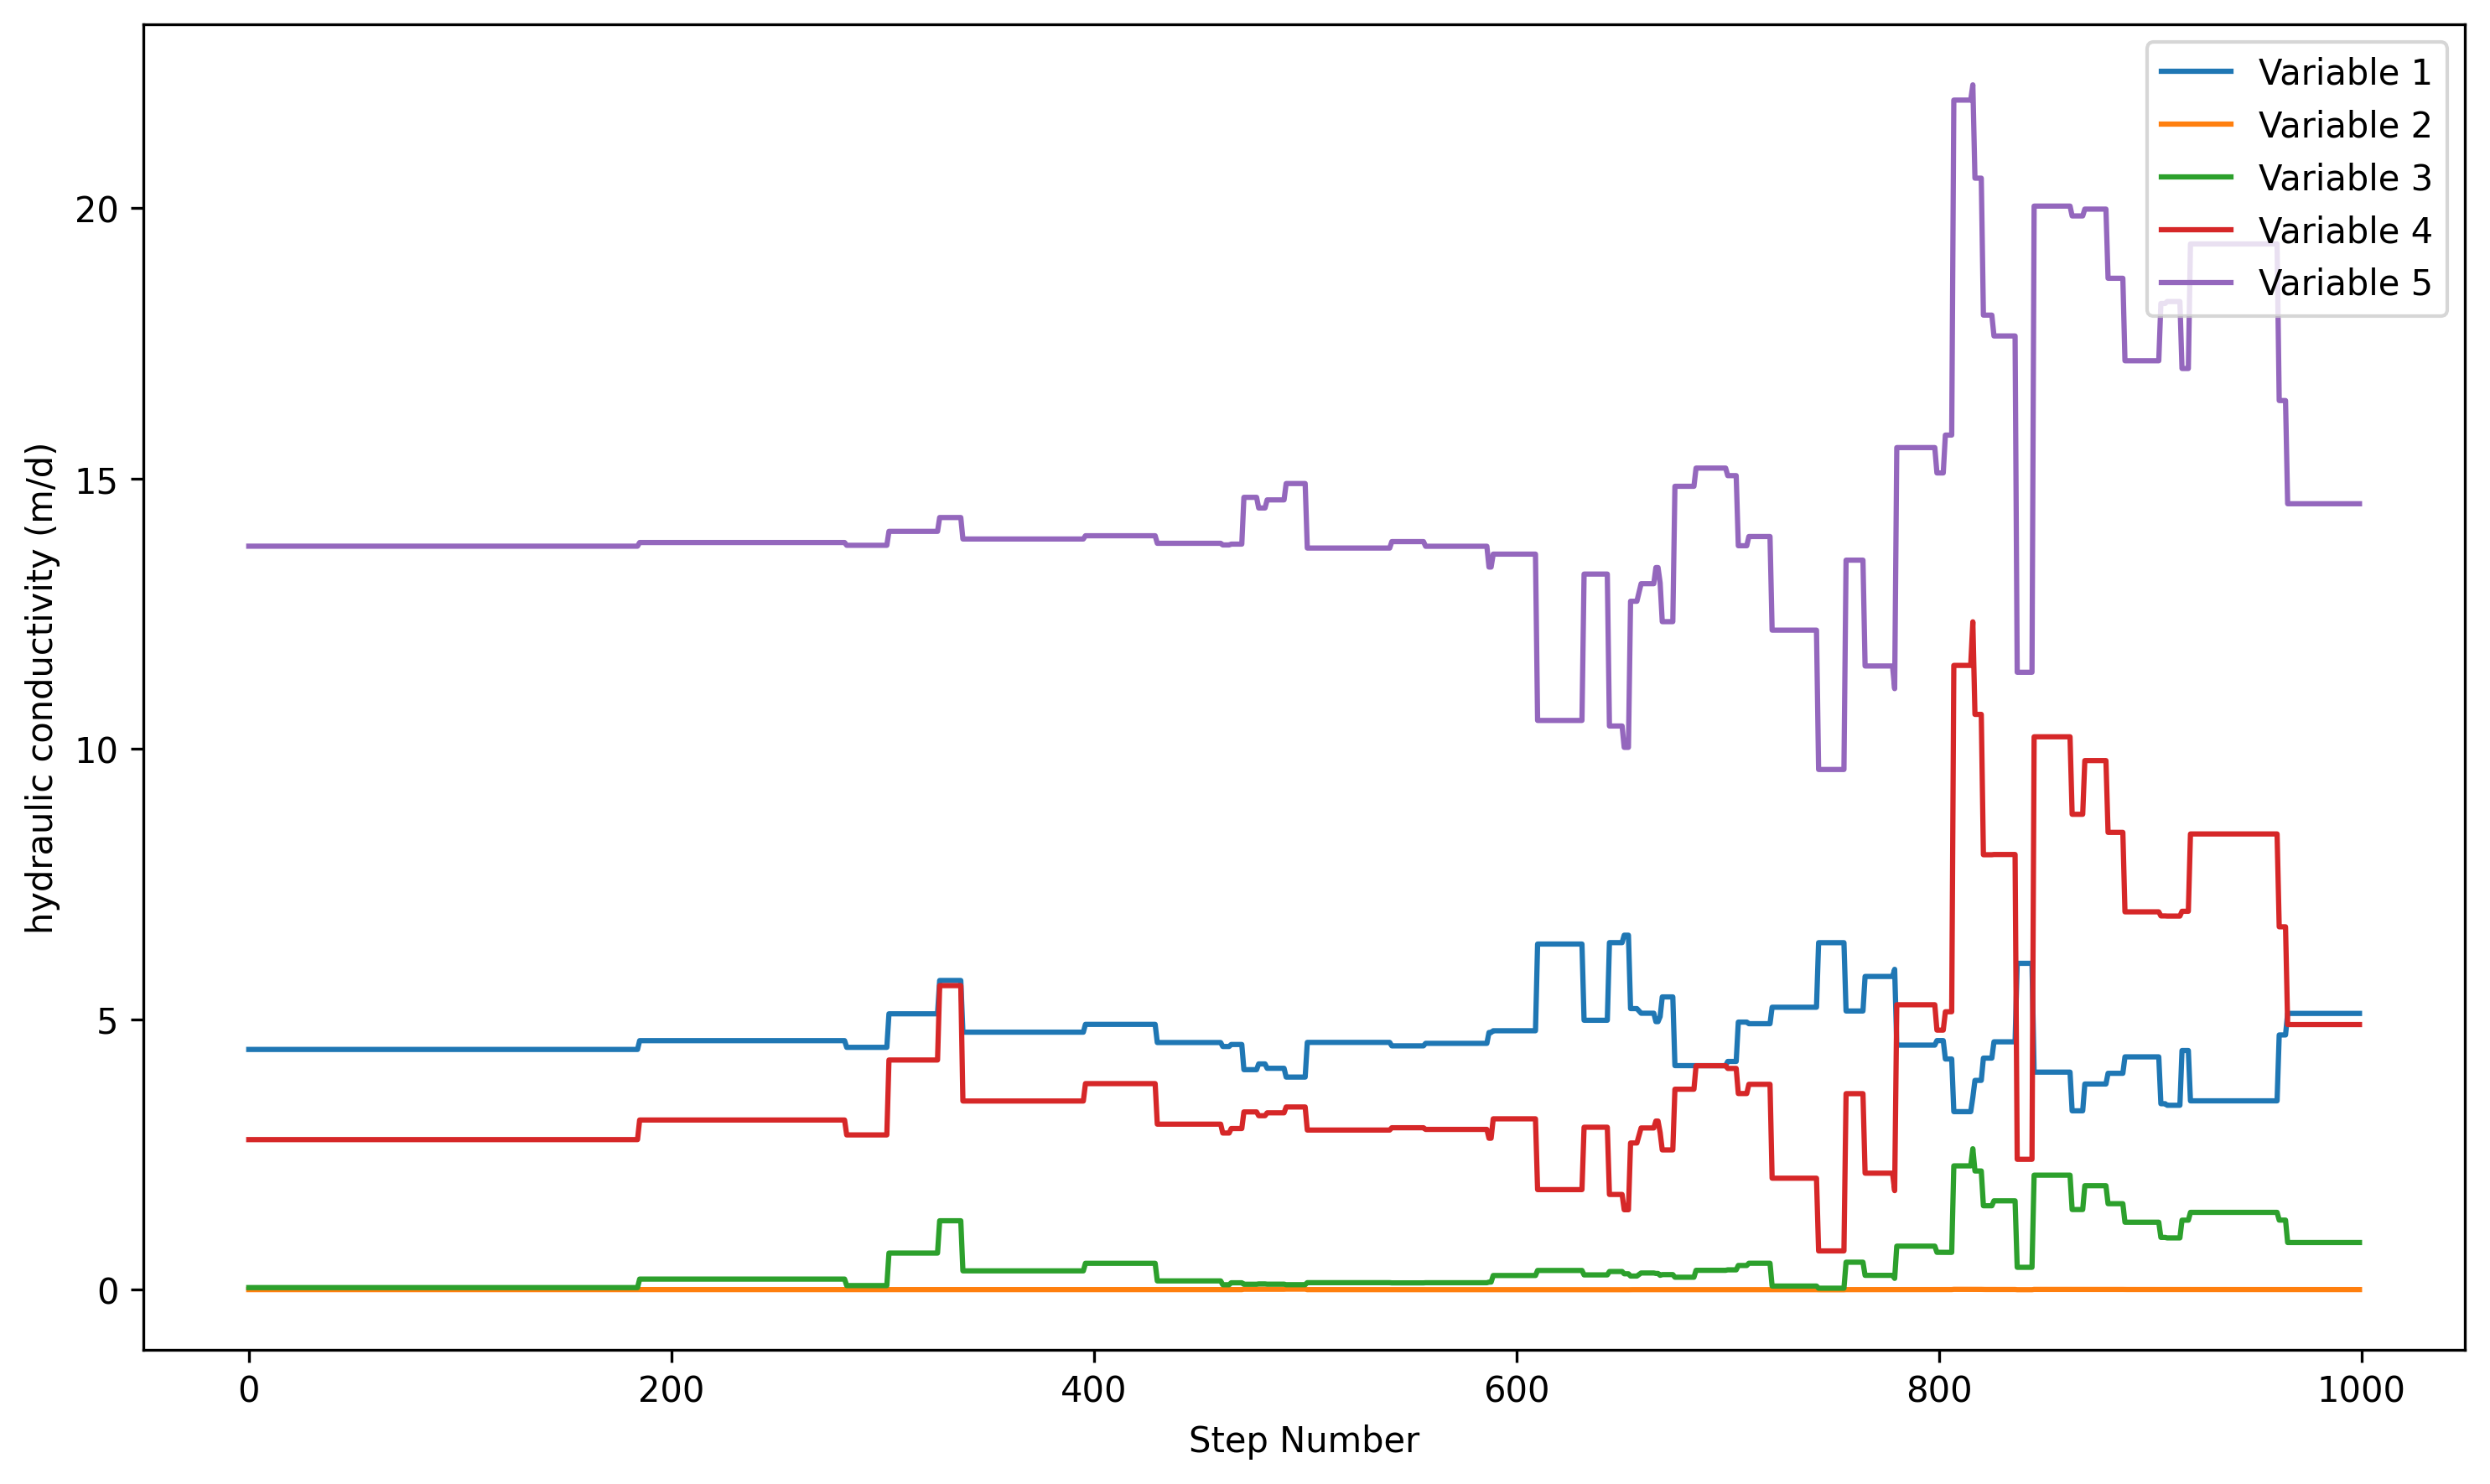
\includegraphics[width=\textwidth]{Figures/appendix_figs/logbook3_trace_plot.png}
\caption{A trace plot of the Stretch move for calibrating model four. The presented chain is the 2\textsuperscript{nd} chain of the 3\textsuperscript{rd}  ensemble. Only the 1000 steps of the main sampling are presented, the 500 burn-in steps were discarded. }\label{fig_logbook_3_trace_plot_Stretch}
\end{figure}